\documentclass{uc3mpracticas}

\usepackage{helvet}
\usepackage{caption}
\usepackage{listings}
\usepackage{multicol}
\renewcommand{\familydefault}{\sfdefault}


%%%%%%%%%%%%%%%%%%%%%%%%%%%%%%%%%%%%%%%%%%%%%%%%%%%%%%%%%%%%%%%%%%%%%%%%%%%%%%%%
%%%                   Plantilla Prácticas UC3M                               %%%
%%%                Universidad Carlos III de Madrid                          %%%
%%%                   Alejandro Valverde Mahou                               %%%
%%%%%%%%%%%%%%%%%%%%%%%%%%%%%%%%%%%%%%%%%%%%%%%%%%%%%%%%%%%%%%%%%%%%%%%%%%%%%%%%

%Permitir cabeceras y pie de páginas personalizados
\pagestyle{fancy}

%Path por defecto de las imágenes
\graphicspath{ {./images/} }

%Declarar formato de encabezado y pie de página de las páginas del documento
\fancypagestyle{doc}{
  %Cabecera
  \headerpr[1]{Planificación Automática}{}{Ingeniería del Conocimiento}
  %Pie de Página
  \footerpr{}{\textbf{UC3M}}{{\thepage} de \pageref{LastPage}}
}

%Declarar formato de encabezado y pie del título e indice
\fancypagestyle{titu}{%
  %Cabecera
  \headerpr{}{}{}
  %Pie de Página
  \footerpr{}{}{}
}


\appto\frontmatter{\pagestyle{titu}}
\appto\mainmatter{\pagestyle{doc}}


\begin{document}
  %Comienzo formato título
  \frontmatter


  %Portada 1 (Centrado todo)
  \centeredtitle{Images/LogoUC3M.png}{Grado en Ingeniería Informática}{Curso 2020/2021}{Ingeniería del Conocimiento}{Práctica 2: Planificación Automática}

  \vspace{55mm}

  \authors{Alba Reinders Sánchez}{100383444}{Alejandro Valverde Mahou}{100383383}{}{}{Grupo 83}{Leganés}

  \newpage

  %Índice
  \tableofcontents

  \newpage

  %Comienzo formato documento general
  \mainmatter

  \section{Introducción}

  En esta segunda práctica se lleva a cabo el modelado de un problema similar al de la práctica anterior pero en este caso un \textbf{planificador} tiene que que simular una sesión entre el robot y el paciente, donde la actividad que realizan es jugar al \textbf{juego de memoria de las cartas}.

  \vspace{2mm}

  El juego planteado al paciente consiste en encontrar parejas de cartas de animales de un conjunto de cartas que están boca abajo. Los jugadores, el robot y el paciente, giran por turnos dos cartas y si la pareja es correcta se dejan boca arriba. Sino se vuelven a girar. Una vez se consigan todas las parejas de una ronda se pasa a la siguiente con otras cartas diferentes.

  \vspace{3mm}

  El documento consiste en el manual técnico con la descripción del dominio implementado, el manual de usuario con la explicación de cómo usar el programa, las pruebas realizadas y el análisis de los resultados, y para finalizar una serie de conclusiones y comentarios personales.

  \vspace{5mm}

  \section{Manual técnico}

  A continuación se describe el dominio creado explicando los \textit{tipos}, los \textit{predicados}, las \textit{funciones} y las \textit{acciones}, en cada acción se especifican sus precondiciones y efectos. Además, se justifican todas las decisiones que se han tenido que tomar durante la implementación.

  \vspace{2mm}

  El flujo de una sesión que se ha planteado es el que se muestra en el siguiente diagrama de estados, donde se pueden ver todas las acciones implementadas para el correcto funcionamiento del planificador.


  \begin{figure}[!h]
    \centering
    \hspace*{-0.75cm}
    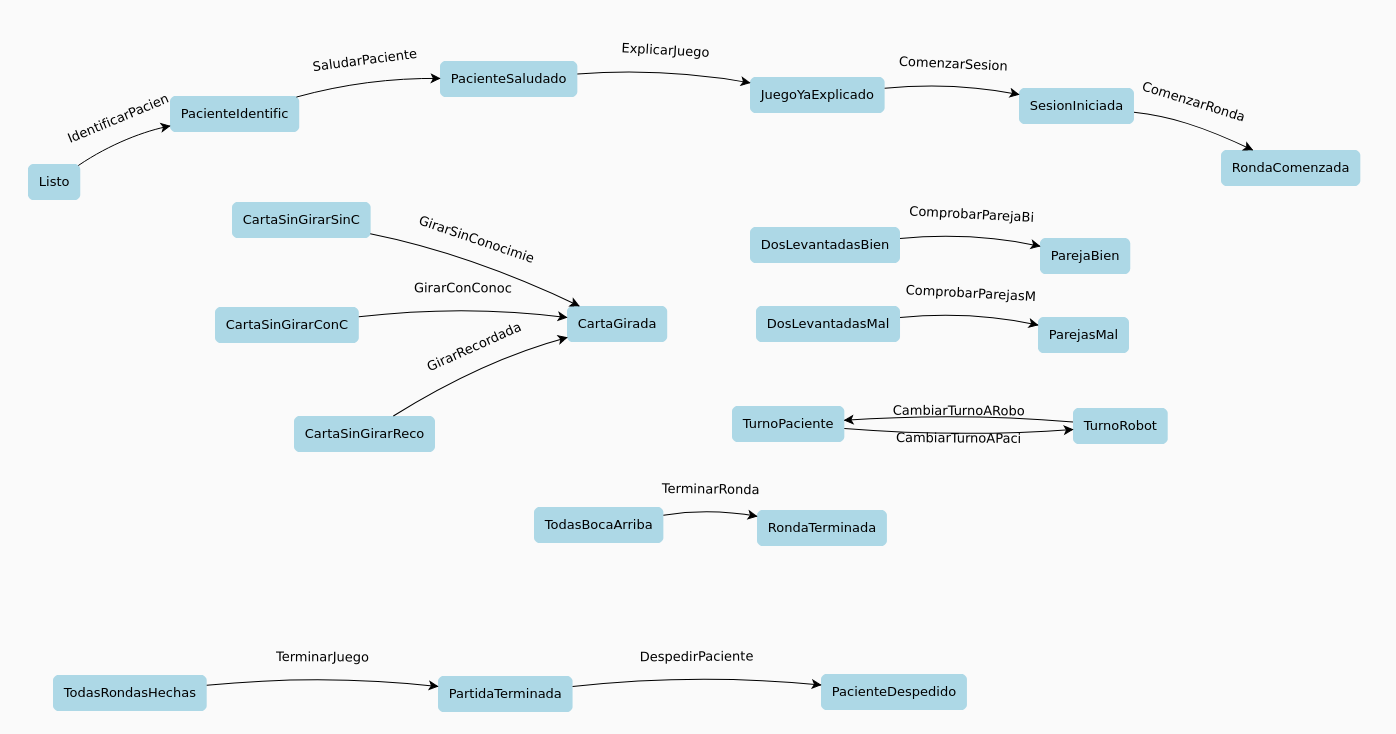
\includegraphics[width=1.1\linewidth]{./Images/flujo.png}
    \caption*{Flujo de una sesión}
  \end{figure}


  \newpage

  \subsection{Tipos}

  Se crean 3 tipos diferentes:

  \begin{itemize}
    \item \textbf{Paciente}: representa el paciente que recibe la sesión. Es necesario crearlo, a diferencia de un tipo 'robot', porque hay que identificar sobre qué paciente se realizan las acciones.
    \item \textbf{Carta}: representa cada una de las cartas del juego. Dado que hay más de una y se aplican diferentes acciones sobre ellas, se tiene que especificar este tipo.
    \item \textbf{Contador}: permite representar los turnos y las rondas. Es un tipo auxiliar.
  \end{itemize}

  \subsection{Predicados}

  Los predicados que se crean para el dominio son los siguientes:

  \begin{itemize}
    \item \textbf{Existe Paciente ?p}: indica el nombre del paciente que va a recibir la sesión. Se usa para reconocer al paciente en el momento inicial.
    \item \textbf{Identificado ?idp}: indica que el paciente ha sido identificado por el robot y por tanto ya se puede proceder a iniciar la sesión.
    \item \textbf{Saludado ?sp}: indica que el paciente ha sido saludado por el robot.
    \item \textbf{JuegoExplicado ?jp}: indica que se le ha explicado el juego al paciente.
    \item \textbf{RondaInicial ?r}: indica el nombre de la ronda inicial. Es necesario usarlo porque es la ronda que da comienzo a toda la sesión.
    \item \textbf{RondaActual ?r}: indica el nombre de la ronda actual de la sesión. Se utiliza como controlador para determinar las cartas que se encuentran en una misma ronda.
    \item \textbf{Siguiente ?r1 ?r2}: indica el orden de las rondas, se pasa de \textit{?r1} a \textit{?r2}.
    \item \textbf{Turno ?t}: indica de quién es el turno. Puede ser del \textit{paciente} o del \textit{nao} (son constantes del dominio).
    \item \textbf{CartaEnRonda ?c ?r}: indica en qué ronda se va a usar cada carta.
    \item \textbf{ParejaCartas ?c1 ?c2}: indica que dos cartas forman una pareja.
    \item \textbf{CartaBocaArriba ?c}: indica que una  carta se encuentra boca arriba. Si la carta se encuentra boca abajo, este predicado no existirá sobre dicha carta.
    \item \textbf{CartaRecordada ?c}: indica que una carta ya ha sido dada la vuelta y es recordada por los jugadores. Se necesita para representar el conocimiento de los jugadores de una forma más cercana a la realidad.
    \item \textbf{CartaEmparejada ?c}: indica que una carta ya ha sido emparejada correctamente.
    \item \textbf{JuegoTerminado}: indica que el juego ha acabado.
    \item \textbf{Despedido ?dp}: indica que el paciente ha sido despedido por el robot. Se propone como el objetivo a cumplir en los problemas.
  \end{itemize}

  \subsection{Funciones}

  Ha sido necesario usar dos funciones auxiliares para representar el dominio correctamente, se trata de dos contadores de cartas:

  \begin{itemize}
    \item \textbf{Contador Boca Arriba}: indica el número de cartas dadas la vuelta y sirve para determinar cuando hay que realizar las comprobaciones. Si tiene un valor de \textit{-1} representa que se ha reseteado para dar fin a un turno o ronda.
    \item \textbf{Contador Recordadas}: indica el número de cartas recordadas por los jugadores y se usa para elegir qué acción de girar carta se debe realizar.
  \end{itemize}


  \subsection{Acciones}

  Respecto a las acciones, se han elaborado todas las necesarias para poder realizar una sesión normal, acciones comunes para ambos jugadores y acciones exclusivas del robot.

  \vspace{2mm}

  Por lo que se van a explicar cada una de las acciones del dominio junto con sus precondiciones y efectos para que sea más clara la explicación.

  \begin{itemize}
    \item \textbf{Identificar Paciente}: acción del robot que permite pasar del estado inicial al momento en el que se ha reconocido al paciente.

      \textit{Precondiciones}: que exista un paciente, y que no haya sido identificado todavía.

      \textit{Efectos}: el paciente pasa a estar identificado.

    \item \textbf{Saludar Paciente}: acción del robot por la que se saluda a un paciente que ya ha sido identificado, antes de empezar un juego.

      \textit{Precondiciones}: que exista un paciente que haya sido identificado, pero no saludado.

      \textit{Efectos}: saludar al paciente.

    \item \textbf{Explicar Juego}: acción del robot en la que este explica las reglas del juego de las cartas.

      \textit{Precondiciones}: que exista un paciente que haya saludado, pero que no se le haya explicado el juego.

      \textit{Efectos}: se le explica el juego al paciente.

    \item \textbf{Comenzar Sesión}: acción del robot que da comienzo al juego.

      \textit{Precondiciones}: que haya un paciente al que se le haya explicado el juego y que exista una ronda inicial.

      \textit{Efectos}: se establece como ronda actual la ronda inicial, se elimina la ronda inicial y se resetea el contador de cartas boca arriba.

    \item \textbf{Comenzar Ronda}: acción del robot que da comienzo a una nueva ronda.

      \textit{Precondiciones}: que exista una ronda actual, que el contador de cartas boca arriba esté reseteado y que no se haya establecido ningún turno.

      \textit{Efectos}: se establece el turno del paciente, se ponen a 0 el contador de cartas boca arriba y el de cartas recordadas.

    \item \textbf{Girar Sin Conocimiento}: acción del robot o del paciente en la que se gira una carta de forma aleatoria porque no se tiene ningún conocimiento previo. Esto sólo se puede hacer si hay menos de dos cartas levantadas en el turno actual.

      \textit{Precondiciones}: que el contador de cartas boca arriba sea 0 o 1, el de cartas recordadas sea 0 y que exista una carta en la ronda actual que no esté boca arriba.

      \textit{Efectos}: la carta pasa a estar boca arriba, aumenta el número de cartas boca arriba y recordadas, y la carta pasa a ser recordada por los jugadores.

    \item \textbf{Girar Con Conocimiento}: acción del robot o del paciente en la que se gira una carta conociendo la posición de alguna otra. Esto sólo se puede hacer si hay menos de dos cartas levantadas en el turno actual.

      \textit{Precondiciones}: que el contador de cartas boca arriba sea 0 o 1, que exista una carta en la ronda actual que no esté boca arriba y que exista otra carta diferente que esté recordada.

      \textit{Efectos}: la carta pasa a estar boca arriba, aumenta el número de cartas boca arriba y recordadas, y la carta pasa a ser recordada por los jugadores.

    \item \textbf{Girar Recordada}: acción del robot o del paciente en la que se gira una carta conociendo la carta previamente. Esto sólo se puede hacer si hay menos de dos cartas levantadas en el turno actual.

      \textit{Precondiciones}: que el contador de cartas boca arriba sea 0 o 1, que haya conocimiento sobre la carta que se va a girar y que esté boca abajo.

      \textit{Efectos}: la carta pasa a estar boca arriba y aumenta el número de cartas boca arriba.

    \item \textbf{Comprobar Pareja Bien}: acción del robot por la que se comprueba que una pareja de cartas boca arriba sea correcta.

      \textit{Precondiciones}: que haya dos cartas boca arriba que no sean la misma, que no estén emparejadas correctamente y que ambas formen una pareja.

      \textit{Efectos}: se resetea el contador de cartas boca arriba y las cartas pasan a estar emparejadas correctamente y dejan de estar recordadas. Se disminuye en 2 el contador de recordadas.

    \item \textbf{Comprobar Pareja Mal}: acción del robot por la que se comprueba que una pareja de cartas boca arriba no sea correcta.

      \textit{Precondiciones}: que haya dos cartas boca arriba que no sean la misma, que no estén emparejadas correctamente y que ambas no formen una pareja.

      \textit{Efectos}: se resetea el contador de cartas boca arriba y las cartas pasan a estar boca abajo.

    \item \textbf{Cambiar Turno A Robot}: acción del robot por la que se cambia de turno al robot una vez haya dos cartas boca arriba.

      \textit{Precondiciones}: que el contador de cartas boca arriba se haya reseteado, que sea el turno del paciente y que siga habiendo cartas boca abajo.

      \textit{Efectos}: pasa a ser el turno del robot y el contador de cartas boca arriba se pone a 0.

    \item \textbf{Cambiar Turno A Paciente}: acción del robot por la que se cambia de turno al paciente una vez haya dos cartas boca arriba.

      \textit{Precondiciones}: que el contador de cartas boca arriba se haya reseteado, que sea el turno del robot y que siga habiendo cartas boca abajo.

      \textit{Efectos}: pasa a ser el turno del paciente y el contador de cartas boca arriba se pone a 0.

    \item \textbf{Terminar Ronda}: acción del robot por la que se termina la ronda actual.

      \textit{Precondiciones}: que el contador de cartas boca arriba se haya reseteado, que no haya cartas de la ronda boca abajo y que exista una ronda siguiente a la actual.

      \textit{Efectos}: la ronda siguiente se convierte en la ronda actual y se eliminan todos los turnos.

    \item \textbf{Terminar Juego}: acción del robot que termina la sesión una vez se han realizado las rondas establecidas.

      \textit{Precondiciones}: que el contador de cartas boca arriba se haya reseteado, que no haya cartas de la ronda boca abajo y que no exista una ronda siguiente a la actual.

      \textit{Efectos}: se termina el juego.

    \item \textbf{Despedir Paciente}: acción del robot que despide al paciente una vez se ha terminado la sesión.

      \textit{Precondiciones}: que la sesión se haya terminado.

      \textit{Efectos}: despedirse del paciente.


  \end{itemize}




  \section{Manual de usuario}

  Para poder ejecutar el programa será necesario ejecutar el siguiente comando:

  \vspace{2mm}

  \begin{lstlisting}
    ~/directorio-cbp/cbp-roller -o domain.pddl -f problema-X.pddl
  \end{lstlisting}

  \vspace{2mm}

  Donde 'X' representa el problema que se quiere ejecutar.

  \vspace{4mm}

  La estructura de cada uno de los problemas es:

  \begin{enumerate}
    \item \textbf{\textit{objects}}:

    En este apartado hay que especificar cada uno de los objetos que se vayan a usar en el problema. Hay que poner el nombre del paciente, el nombre de las rondas y el nombre de cada carta.

    \item \textbf{\textit{init}}:

    En este apartado hay que especificar todos los predicados necesarios. Hay que establecer el nombre de la ronda inicial, el orden de las rondas, a qué ronda pertenece cada carta, las parejas de cartas y el nombre del paciente que va a recibir la sesión.

    \item \textbf{\textit{goal}}:

    Por último, se especifica el objetivo a cumplir del problema. Suele ser \textbf{(Despedido \textit{nombre\_paciente})}, que representa el final de una sesión ejecutada con normalidad.

  \end{enumerate}



  \section{Pruebas realizadas}

  Con el fin de comprobar el funcionamiento correcto del dominio desarrollado, se crean una serie de problemas con estados iniciales y complejidad variable. Se va a hacer una breve descripción de las pruebas realizadas y se analizarán los resultados obtenidos.

  \subsection{Prueba 1}

  Esta prueba representa el caso base donde se tienen 6 cartas por ronda y hay un total de 2 rondas. El objetivo de la prueba es realizar una ejecución normal del código para demostrar que funciona correctamente.

  \begin{multicols}{2}
    \textbf{Plan obtenido}:

    \begin{lstlisting}
0: (IDENTIFICAR_PACIENTE TEO)
1: (SALUDAR_PACIENTE TEO)
2: (EXPLICAR_JUEGO TEO)
3: (COMENZAR_SESION TEO GRANJA)
4: (COMENZAR_RONDA GRANJA)
5: (GIRAR_SIN_CONOCIMIENTO CERDO1 GRANJA)
6: (GIRAR_CON_CONOCIMIENTO CERDO2 CERDO1 GRANJA)
7: (COMPROBAR_PAREJA_BIEN CERDO2 CERDO1 GRANJA)
8: (CAMBIAR_TURNO_A_ROBOT)
9: (GIRAR_SIN_CONOCIMIENTO VACA1 GRANJA)
10: (GIRAR_CON_CONOCIMIENTO VACA2 VACA1 GRANJA)
11: (COMPROBAR_PAREJA_BIEN VACA2 VACA1 GRANJA)
12: (CAMBIAR_TURNO_A_PACIENTE)
13: (GIRAR_SIN_CONOCIMIENTO CABALLO1 GRANJA)
14: (GIRAR_CON_CONOCIMIENTO CABALLO2 CABALLO1 GRANJA)
15: (COMPROBAR_PAREJA_BIEN CABALLO2 CABALLO1 GRANJA)
16: (TERMINAR_RONDA GRANJA JUNGLA)
17: (COMENZAR_RONDA JUNGLA)
18: (GIRAR_SIN_CONOCIMIENTO MONO1 JUNGLA)
19: (GIRAR_CON_CONOCIMIENTO MONO2 MONO1 JUNGLA)
20: (COMPROBAR_PAREJA_BIEN MONO2 MONO1 JUNGLA)
21: (CAMBIAR_TURNO_A_ROBOT)
22: (GIRAR_SIN_CONOCIMIENTO SERPIENTE1 JUNGLA)
23: (GIRAR_CON_CONOCIMIENTO SERPIENTE2 SERPIENTE1 JUNGLA)
24: (COMPROBAR_PAREJA_BIEN SERPIENTE2 SERPIENTE1 JUNGLA)
25: (CAMBIAR_TURNO_A_PACIENTE)
26: (GIRAR_SIN_CONOCIMIENTO TIGRE1 JUNGLA)
27: (GIRAR_CON_CONOCIMIENTO TIGRE2 TIGRE1 JUNGLA)
28: (COMPROBAR_PAREJA_BIEN TIGRE2 TIGRE1 JUNGLA)
29: (TERMINAR_JUEGO JUNGLA)
30: (DESPEDIR_PACIENTE TEO)
    \end{lstlisting}

    \columnbreak

    \textbf{Fichero del problema}: problema-1.pddl

    \textbf{Fichero del resultado}: problema-1-o.pddl

    \textbf{Tiempo de ejecución}: 0.00 segundos
  \end{multicols}

  Los resultados obtenidos son los esperados, el planificador resuelve el problema de forma correcta. Sin embargo, cabe destacar que el el plan generado no parece una ejecución normal del juego de las cartas, ya que siempre aciertan las parejas a la primera. Esto se debe a que el planificador intenta conseguir el plan con menor longitud (al no haberse especificado otra métrica) y este es el que se consigue cuando se acierta todo a la primera.

  \vspace{2mm}

  Para conseguir planes más semejantes a la realidad, en otras pruebas se van a pedir requisitos adicionales con el fin de forzar al planificador a crear planes más realistas.

  \vspace{2mm}

  Además, en este caso no se puede asegurar el funcionamiento de todas las acciones ya que algunas de ellas, como por ejemplo \textit{Comprobar Pareja Mal}, nunca van a ejecutarse.


  \newpage

  \subsection{Prueba 2}

  Esta prueba pretende conseguir una ejecución más realista usando un contador de errores que requiere que el plan realice al menos 3 errores. El resto es igual que la prueba anterior: se tienen 6 cartas por ronda y hay un total de 2 rondas.

  \vspace{2mm}

  Para implementar este contador de errores se añade en funciones \textit{Contador Errores} y en los efectos de la acción \textit{Comenzar Sesion} que se ponga el contador a 0, y en los de \textit{Comprobar Pareja Mal} se añade 1 al contador.

  \vspace{2mm}

  De esta forma se obliga al planificador a pasar 3 veces por la acción que representa una equivocación.

  \begin{multicols}{2}
    \textbf{Plan obtenido}:

    \begin{lstlisting}
0: (IDENTIFICAR_PACIENTE TEO)
1: (SALUDAR_PACIENTE TEO)
2: (EXPLICAR_JUEGO TEO)
3: (COMENZAR_SESION TEO GRANJA)
4: (COMENZAR_RONDA GRANJA)
5: (GIRAR_SIN_CONOCIMIENTO CERDO2 GRANJA)
6: (GIRAR_CON_CONOCIMIENTO CABALLO2 CERDO2 GRANJA)
7: (COMPROBAR_PAREJA_MAL CABALLO2 CERDO2 GRANJA)
8: (CAMBIAR_TURNO_A_ROBOT)
9: (GIRAR_RECORDADA GRANJA CERDO2)
10: (GIRAR_RECORDADA GRANJA CABALLO2)
11: (COMPROBAR_PAREJA_MAL CABALLO2 CERDO2 GRANJA)
12: (CAMBIAR_TURNO_A_PACIENTE)
13: (GIRAR_RECORDADA GRANJA CERDO2)
14: (GIRAR_RECORDADA GRANJA CABALLO2)
15: (COMPROBAR_PAREJA_MAL CABALLO2 CERDO2 GRANJA)
16: (CAMBIAR_TURNO_A_ROBOT)
17: (GIRAR_RECORDADA GRANJA CERDO2)
18: (GIRAR_CON_CONOCIMIENTO CERDO1 CABALLO2 GRANJA)
19: (COMPROBAR_PAREJA_BIEN CERDO2 CERDO1 GRANJA)
20: (CAMBIAR_TURNO_A_PACIENTE)
21: (GIRAR_CON_CONOCIMIENTO VACA1 CABALLO2 GRANJA)
22: (GIRAR_CON_CONOCIMIENTO VACA2 CABALLO2 GRANJA)
23: (COMPROBAR_PAREJA_BIEN VACA2 VACA1 GRANJA)
24: (CAMBIAR_TURNO_A_ROBOT)
25: (GIRAR_CON_CONOCIMIENTO CABALLO1 CABALLO2 GRANJA)
26: (GIRAR_RECORDADA GRANJA CABALLO2)
27: (COMPROBAR_PAREJA_BIEN CABALLO2 CABALLO1 GRANJA)
28: (TERMINAR_RONDA GRANJA JUNGLA)
29: (COMENZAR_RONDA JUNGLA)
30: (GIRAR_SIN_CONOCIMIENTO MONO1 JUNGLA)
31: (GIRAR_CON_CONOCIMIENTO MONO2 MONO1 JUNGLA)
32: (COMPROBAR_PAREJA_BIEN MONO2 MONO1 JUNGLA)
33: (CAMBIAR_TURNO_A_ROBOT)
34: (GIRAR_SIN_CONOCIMIENTO SERPIENTE1 JUNGLA)
35: (GIRAR_CON_CONOCIMIENTO SERPIENTE2 SERPIENTE1 JUNGLA)
36: (COMPROBAR_PAREJA_BIEN SERPIENTE2 SERPIENTE1 JUNGLA)
37: (CAMBIAR_TURNO_A_PACIENTE)
38: (GIRAR_SIN_CONOCIMIENTO TIGRE1 JUNGLA)
39: (GIRAR_CON_CONOCIMIENTO TIGRE2 TIGRE1 JUNGLA)
40: (COMPROBAR_PAREJA_BIEN TIGRE2 TIGRE1 JUNGLA)
41: (TERMINAR_JUEGO JUNGLA)
42: (DESPEDIR_PACIENTE TEO)
    \end{lstlisting}

    \columnbreak

    \textbf{Fichero del problema}: problema-2.pddl

    \textbf{Fichero del resultado}: problema-2-o.pddl

    \textbf{Tiempo de ejecución}: 0.01 segundos
  \end{multicols}

  A pesar de que los resultados obtenidos sí concuerdan con los esperados, siguen sin ser ejecuciones que se puedan parecer a las reales, porque lo que hace el planificador es equivocarse levantando las mismas cartas 3 veces seguidas al principio, y depués el resto de turnos los hace perfectos, igual que en la prueba anterior.

  \vspace{2mm}

  Aún así permite probar las acciones que antes no se podía, porque se fuerza su aparición.


  \subsection{Prueba 3}

  Con esta prueba se quiere crear y probar una interrupción sobre la sesión. En este caso esta interrupción consiste en que antes de que empiece una ronda haya algunas cartas boca arriba. Para ello se tiene que crear una nueva acción:

  \vspace{2mm}

  \textbf{Colocar Mal Giradas}: acción del robot que coloca todas las cartas boca abajo antes de empezar una ronda.

  \vspace{1mm}

    \textit{Precondiciones}: que exista una ronda actual, que el contador de cartas boca arriba esté reseteado, que no se haya establecido ningún turno y que haya alguna carta boca arriba.

    \vspace{1mm}

    \textit{Efectos}: se da la vuelta a la carta boca arriba.


  \vspace{2mm}

  Además, se tiene que añadir la precondición de que no haya ninguna carta boca arriba antes de empezar una ronda en la acción \textit{Comenzar Ronda}.

  \vspace{3mm}

  En este problema se tienen 4 cartas por ronda y hay un total de 2 rondas. Hay una carta levantada en cada ronda.



  \begin{multicols}{2}
    \textbf{Plan obtenido}:

    \begin{lstlisting}
0: (IDENTIFICAR_PACIENTE TEO)
1: (SALUDAR_PACIENTE TEO)
2: (EXPLICAR_JUEGO TEO)
3: (COMENZAR_SESION TEO GRANJA)
4: (COLOCAR_MAL_GIRADAS GRANJA VACA2)
5: (COMENZAR_RONDA GRANJA)
6: (GIRAR_SIN_CONOCIMIENTO VACA1 GRANJA)
7: (GIRAR_CON_CONOCIMIENTO VACA2 VACA1 GRANJA)
8: (COMPROBAR_PAREJA_BIEN VACA2 VACA1 GRANJA)
9: (CAMBIAR_TURNO_A_ROBOT)
10: (GIRAR_SIN_CONOCIMIENTO CABALLO1 GRANJA)
11: (GIRAR_CON_CONOCIMIENTO CABALLO2 CABALLO1 GRANJA)
12: (COMPROBAR_PAREJA_BIEN CABALLO2 CABALLO1 GRANJA)
13: (TERMINAR_RONDA GRANJA JUNGLA)
14: (COLOCAR_MAL_GIRADAS JUNGLA TIGRE1)
15: (COMENZAR_RONDA JUNGLA)
16: (GIRAR_SIN_CONOCIMIENTO SERPIENTE1 JUNGLA)
17: (GIRAR_CON_CONOCIMIENTO SERPIENTE2 SERPIENTE1 JUNGLA)
18: (COMPROBAR_PAREJA_BIEN SERPIENTE2 SERPIENTE1 JUNGLA)
19: (CAMBIAR_TURNO_A_ROBOT)
20: (GIRAR_SIN_CONOCIMIENTO TIGRE1 JUNGLA)
21: (GIRAR_CON_CONOCIMIENTO TIGRE2 TIGRE1 JUNGLA)
22: (COMPROBAR_PAREJA_BIEN TIGRE2 TIGRE1 JUNGLA)
23: (TERMINAR_JUEGO JUNGLA)
24: (DESPEDIR_PACIENTE TEO)
    \end{lstlisting}

    \columnbreak

    \textbf{Fichero del problema}: problema-3.pddl

    \textbf{Fichero del resultado}: problema-3-o.pddl

    \textbf{Tiempo de ejecución}: 0.00 segundos
  \end{multicols}

  El planificador consigue resolver correctamente el problema corrigiendo antes de empezar cada ronda las cartas que están boca arriba al inicio de una ronda.


  \subsection{Prueba 4}

  Esta prueba pretende probar una interrupción sobre la sesión que consiste en que el paciente es despistado y no se entera de la explicación del juego y por tanto hay que explicarsela de nuevo. Para ello se crea una nueva acción:

  \vspace{2mm}

  \textbf{Explicar Juego Despistado}: acción del robot que vuelve a explicar el juego al paciente despistado.

  \vspace{1mm}

    \textit{Precondiciones}: que el juego ya haya sido explicado y que el paciente sea despistado.

    \vspace{1mm}

    \textit{Efectos}: se puede iniciar el juego.


  \vspace{2mm}

  Además, se tiene que añadir el predicado \textit{(Despistado ?p - Paciente)} y la precondición de que el paciente no esté despistado en la acción \textit{Comenzar Sesion}.

  \vspace{3mm}

  En este problema se tienen 4 cartas por ronda y hay un total de 2 rondas. El paciente está despistado.

  \begin{multicols}{2}
    \textbf{Plan obtenido}:

    \begin{lstlisting}
0: (IDENTIFICAR_PACIENTE TEO)
1: (SALUDAR_PACIENTE TEO)
2: (EXPLICAR_JUEGO TEO)
3: (EXPLICAR_JUEGO_DESPISTADO TEO)
4: (COMENZAR_SESION TEO GRANJA)
5: (COMENZAR_RONDA GRANJA)
6: (GIRAR_SIN_CONOCIMIENTO VACA1 GRANJA)
7: (GIRAR_CON_CONOCIMIENTO VACA2 VACA1 GRANJA)
8: (COMPROBAR_PAREJA_BIEN VACA2 VACA1 GRANJA)
9: (CAMBIAR_TURNO_A_ROBOT)
10: (GIRAR_SIN_CONOCIMIENTO CABALLO1 GRANJA)
11: (GIRAR_CON_CONOCIMIENTO CABALLO2 CABALLO1 GRANJA)
12: (COMPROBAR_PAREJA_BIEN CABALLO2 CABALLO1 GRANJA)
13: (TERMINAR_RONDA GRANJA JUNGLA)
14: (COMENZAR_RONDA JUNGLA)
15: (GIRAR_SIN_CONOCIMIENTO SERPIENTE1 JUNGLA)
16: (GIRAR_CON_CONOCIMIENTO SERPIENTE2 SERPIENTE1 JUNGLA)
17: (COMPROBAR_PAREJA_BIEN SERPIENTE2 SERPIENTE1 JUNGLA)
18: (CAMBIAR_TURNO_A_ROBOT)
19: (GIRAR_SIN_CONOCIMIENTO TIGRE1 JUNGLA)
20: (GIRAR_CON_CONOCIMIENTO TIGRE2 TIGRE1 JUNGLA)
21: (COMPROBAR_PAREJA_BIEN TIGRE2 TIGRE1 JUNGLA)
22: (TERMINAR_JUEGO JUNGLA)
23: (DESPEDIR_PACIENTE TEO)
    \end{lstlisting}

    \columnbreak

    \textbf{Fichero del problema}: problema-4.pddl

    \textbf{Fichero del resultado}: problema-4-o.pddl

    \textbf{Tiempo de ejecución}: 0.00 segundos
  \end{multicols}

  Se puede ver en plan que el planificador resuelve el problema explicando dos veces el juego.

  \newpage

  \subsection{Prueba 5}

  Esta prueba representa una sesión con más cartas y más rondas, por lo que se quiere probar que se pueden resolver problemas más complejos correctamente.

  \vspace{3mm}

  Por lo tanto, para este problema se tienen 8 cartas por ronda y hay un total de 4 rondas.

  \vspace{3mm}

    \textbf{Plan obtenido}:

    \begin{lstlisting}
0: (IDENTIFICAR_PACIENTE TEO)
1: (SALUDAR_PACIENTE TEO)
2: (EXPLICAR_JUEGO TEO)
3: (COMENZAR_SESION TEO GRANJA)
4: (COMENZAR_RONDA GRANJA)
5: (GIRAR_SIN_CONOCIMIENTO CERDO1 GRANJA)
6: (GIRAR_CON_CONOCIMIENTO CERDO2 CERDO1 GRANJA)
7: (COMPROBAR_PAREJA_BIEN CERDO2 CERDO1 GRANJA)
8: (CAMBIAR_TURNO_A_ROBOT)
9: (GIRAR_SIN_CONOCIMIENTO VACA1 GRANJA)
10: (GIRAR_CON_CONOCIMIENTO VACA2 VACA1 GRANJA)
11: (COMPROBAR_PAREJA_BIEN VACA2 VACA1 GRANJA)
12: (CAMBIAR_TURNO_A_PACIENTE)
13: (GIRAR_SIN_CONOCIMIENTO CABALLO1 GRANJA)
14: (GIRAR_CON_CONOCIMIENTO CABALLO2 CABALLO1 GRANJA)
15: (COMPROBAR_PAREJA_BIEN CABALLO2 CABALLO1 GRANJA)
16: (CAMBIAR_TURNO_A_ROBOT)
17: (GIRAR_SIN_CONOCIMIENTO PATO1 GRANJA)
18: (GIRAR_CON_CONOCIMIENTO PATO2 PATO1 GRANJA)
19: (COMPROBAR_PAREJA_BIEN PATO2 PATO1 GRANJA)
20: (TERMINAR_RONDA GRANJA JUNGLA)
21: (COMENZAR_RONDA JUNGLA)
22: (GIRAR_SIN_CONOCIMIENTO MONO1 JUNGLA)
23: (GIRAR_CON_CONOCIMIENTO MONO2 MONO1 JUNGLA)
24: (COMPROBAR_PAREJA_BIEN MONO2 MONO1 JUNGLA)
25: (CAMBIAR_TURNO_A_ROBOT)
26: (GIRAR_SIN_CONOCIMIENTO SERPIENTE1 JUNGLA)
27: (GIRAR_CON_CONOCIMIENTO SERPIENTE2 SERPIENTE1 JUNGLA)
28: (COMPROBAR_PAREJA_BIEN SERPIENTE2 SERPIENTE1 JUNGLA)
29: (CAMBIAR_TURNO_A_PACIENTE)
30: (GIRAR_SIN_CONOCIMIENTO TIGRE1 JUNGLA)
31: (GIRAR_CON_CONOCIMIENTO TIGRE2 TIGRE1 JUNGLA)
32: (COMPROBAR_PAREJA_BIEN TIGRE2 TIGRE1 JUNGLA)
33: (CAMBIAR_TURNO_A_ROBOT)
34: (GIRAR_SIN_CONOCIMIENTO LORO1 JUNGLA)
35: (GIRAR_CON_CONOCIMIENTO LORO2 LORO1 JUNGLA)
36: (COMPROBAR_PAREJA_BIEN LORO2 LORO1 JUNGLA)
37: (TERMINAR_RONDA JUNGLA MAR)
38: (COMENZAR_RONDA MAR)
39: (GIRAR_SIN_CONOCIMIENTO DELFIN1 MAR)
40: (GIRAR_CON_CONOCIMIENTO DELFIN2 DELFIN1 MAR)
41: (COMPROBAR_PAREJA_BIEN DELFIN2 DELFIN1 MAR)
42: (CAMBIAR_TURNO_A_ROBOT)
43: (GIRAR_SIN_CONOCIMIENTO PEZ1 MAR)
44: (GIRAR_CON_CONOCIMIENTO PEZ2 PEZ1 MAR)
45: (COMPROBAR_PAREJA_BIEN PEZ2 PEZ1 MAR)
46: (CAMBIAR_TURNO_A_PACIENTE)
47: (GIRAR_SIN_CONOCIMIENTO TIBURON1 MAR)
48: (GIRAR_CON_CONOCIMIENTO TIBURON2 TIBURON1 MAR)
49: (COMPROBAR_PAREJA_BIEN TIBURON2 TIBURON1 MAR)
50: (CAMBIAR_TURNO_A_ROBOT)
51: (GIRAR_SIN_CONOCIMIENTO PULPO1 MAR)
52: (GIRAR_CON_CONOCIMIENTO PULPO2 PULPO1 MAR)
53: (COMPROBAR_PAREJA_BIEN PULPO2 PULPO1 MAR)
54: (TERMINAR_RONDA MAR DESIERTO)
55: (COMENZAR_RONDA DESIERTO)
56: (GIRAR_SIN_CONOCIMIENTO ESCORPION1 DESIERTO)
57: (GIRAR_CON_CONOCIMIENTO ESCORPION2 ESCORPION1 DESIERTO)
58: (COMPROBAR_PAREJA_BIEN ESCORPION2 ESCORPION1 DESIERTO)
59: (CAMBIAR_TURNO_A_ROBOT)
60: (GIRAR_SIN_CONOCIMIENTO CAMELLO1 DESIERTO)
61: (GIRAR_CON_CONOCIMIENTO CAMELLO2 CAMELLO1 DESIERTO)
62: (COMPROBAR_PAREJA_BIEN CAMELLO2 CAMELLO1 DESIERTO)
63: (CAMBIAR_TURNO_A_PACIENTE)
64: (GIRAR_SIN_CONOCIMIENTO COYOTE1 DESIERTO)
65: (GIRAR_CON_CONOCIMIENTO COYOTE2 COYOTE1 DESIERTO)
66: (COMPROBAR_PAREJA_BIEN COYOTE2 COYOTE1 DESIERTO)
67: (CAMBIAR_TURNO_A_ROBOT)
68: (GIRAR_SIN_CONOCIMIENTO HORMIGA1 DESIERTO)
69: (GIRAR_CON_CONOCIMIENTO HORMIGA2 HORMIGA1 DESIERTO)
70: (COMPROBAR_PAREJA_BIEN HORMIGA2 HORMIGA1 DESIERTO)
71: (TERMINAR_JUEGO DESIERTO)
72: (DESPEDIR_PACIENTE TEO)
    \end{lstlisting}

    \vspace{2mm}

    \textbf{Fichero del problema}: problema-5.pddl

    \textbf{Fichero del resultado}: problema-5-o.pddl

    \textbf{Tiempo de ejecución}: 0.06 segundos

    \vspace{3mm}

  Los resultados obtenidos son los esperados, funciona correctamente a pesar de que se haya aumentado la complejidad.

  \newpage

  \subsection{Prueba 6}

  Con esta última prueba se pretende probar el comportamiento cuando se mezclan el número de errores mínimos requeridos, que el paciente esté despistado y que haya cartas boca arriba al inicio de cada ronda.

  \vspace{3mm}

  En este problema se tienen 6 cartas por ronda y hay un total de 2 rondas. El paciente está despistado y hay 2 cartas boca arriba en cada ronda. Además, se fuerza a que se produzcan 3 equivocaciones.

  \vspace{3mm}

    \textbf{Plan obtenido}:

    \begin{lstlisting}
0: (IDENTIFICAR_PACIENTE TEO)
1: (SALUDAR_PACIENTE TEO)
2: (EXPLICAR_JUEGO TEO)
3: (EXPLICAR_JUEGO_DESPISTADO TEO)
4: (COMENZAR_SESION TEO GRANJA)
5: (COLOCAR_MAL_GIRADAS GRANJA VACA2)
6: (COLOCAR_MAL_GIRADAS GRANJA CABALLO1)
7: (COMENZAR_RONDA GRANJA)
8: (GIRAR_SIN_CONOCIMIENTO CERDO2 GRANJA)
9: (GIRAR_CON_CONOCIMIENTO CABALLO2 CERDO2 GRANJA)
10: (COMPROBAR_PAREJA_MAL CABALLO2 CERDO2 GRANJA)
11: (CAMBIAR_TURNO_A_ROBOT)
12: (GIRAR_RECORDADA GRANJA CERDO2)
13: (GIRAR_RECORDADA GRANJA CABALLO2)
14: (COMPROBAR_PAREJA_MAL CABALLO2 CERDO2 GRANJA)
15: (CAMBIAR_TURNO_A_PACIENTE)
16: (GIRAR_RECORDADA GRANJA CERDO2)
17: (GIRAR_RECORDADA GRANJA CABALLO2)
18: (COMPROBAR_PAREJA_MAL CABALLO2 CERDO2 GRANJA)
19: (CAMBIAR_TURNO_A_ROBOT)
20: (GIRAR_RECORDADA GRANJA CERDO2)
21: (GIRAR_CON_CONOCIMIENTO CERDO1 CABALLO2 GRANJA)
22: (COMPROBAR_PAREJA_BIEN CERDO2 CERDO1 GRANJA)
23: (CAMBIAR_TURNO_A_PACIENTE)
24: (GIRAR_CON_CONOCIMIENTO VACA1 CABALLO2 GRANJA)
25: (GIRAR_CON_CONOCIMIENTO VACA2 CABALLO2 GRANJA)
26: (COMPROBAR_PAREJA_BIEN VACA2 VACA1 GRANJA)
27: (CAMBIAR_TURNO_A_ROBOT)
28: (GIRAR_CON_CONOCIMIENTO CABALLO1 CABALLO2 GRANJA)
29: (GIRAR_RECORDADA GRANJA CABALLO2)
30: (COMPROBAR_PAREJA_BIEN CABALLO2 CABALLO1 GRANJA)
31: (TERMINAR_RONDA GRANJA JUNGLA)
32: (COLOCAR_MAL_GIRADAS JUNGLA MONO2)
33: (COLOCAR_MAL_GIRADAS JUNGLA SERPIENTE2)
34: (COMENZAR_RONDA JUNGLA)
35: (GIRAR_SIN_CONOCIMIENTO MONO1 JUNGLA)
36: (GIRAR_CON_CONOCIMIENTO MONO2 MONO1 JUNGLA)
37: (COMPROBAR_PAREJA_BIEN MONO2 MONO1 JUNGLA)
38: (CAMBIAR_TURNO_A_ROBOT)
39: (GIRAR_SIN_CONOCIMIENTO SERPIENTE1 JUNGLA)
40: (GIRAR_CON_CONOCIMIENTO SERPIENTE2 SERPIENTE1 JUNGLA)
41: (COMPROBAR_PAREJA_BIEN SERPIENTE2 SERPIENTE1 JUNGLA)
42: (CAMBIAR_TURNO_A_PACIENTE)
43: (GIRAR_SIN_CONOCIMIENTO TIGRE1 JUNGLA)
44: (GIRAR_CON_CONOCIMIENTO TIGRE2 TIGRE1 JUNGLA)
45: (COMPROBAR_PAREJA_BIEN TIGRE2 TIGRE1 JUNGLA)
46: (TERMINAR_JUEGO JUNGLA)
47: (DESPEDIR_PACIENTE TEO)

    \end{lstlisting}

    \vspace{2mm}

    \textbf{Fichero del problema}: problema-6.pddl

    \textbf{Fichero del resultado}: problema-6-o.pddl

    \textbf{Tiempo de ejecución}: 0.01 segundos

  \vspace{3mm}

  El planificador resuelve satisfactoriamente el problema manejando todas las distintas modificaciones de forma correcta.


  \section{Conclusiones}

  Esta práctica ha servido para afianzar los conocimientos sobre planificadores aprendidos en clase, teniendo que crear un dominio y una serie de problemas, con los distintos pasos que ello conlleva.

  \vspace{2mm}

  El dominio sobre el que se ha trabajado es para una sesión del juego de memoria de emparejar cartas de animales. A pesar de que se consigue un flujo que resuelve el problema, no parece una sesión 'real' dado que, como lo resuelve lo más rápido posible a falta de otra métrica, siempre adivina las parejas a la primera. Si fuera una sesión 'real' lo normal sería que ambos jugadores se equivocaran al hacer las parejas más de una vez.

  \section{Comentarios personales}

  El principal problema encontrado ha sido durante el uso de la herramienta proporcionada para crear el diagrama de flujo, ya que tenía algunos fallos como que no se podía guardar el diagrama creado para modificarlo después.

  \vspace{2mm}

  Una vez generados los archivos \textit{.pddl} con el programa fue necesario modificar prácticamente todas las acciones.

  \vspace{2mm}

  A parte de esto, no ha habido mayores dificultades, quitando algunos errores en la conceptualización del dominio pero que han sido resueltos gracias a las diferentes pruebas creadas.



\end{document}
